\documentclass[12pt,a4paper]{article}
\usepackage[utf8]{inputenc}
\usepackage[czech]{babel}
\usepackage[T1]{fontenc}
\usepackage{float}
\usepackage{graphicx}
\usepackage{hyperref}
\usepackage{index}
\usepackage{listings}
\usepackage{url}
\usepackage{enumitem}
\usepackage[left=3.5cm,right=2.5cm,top=2.5cm,bottom=2.5cm]{geometry}
\author{Roman Ondráček}
\title{Měření a regulace teploty v domácnosti}
% Vytvoření seznamu použitých zkratek
\newindex{zkr}{zdx}{znd}{Seznam použitých zkratek}
\setlist{nolistsep}
\lstset{
  inputencoding=utf8
}
\begin{document}
% Řádkování 1,5
\renewcommand{\baselinestretch}{1.5}
% Vynechání číslování
\pagestyle{empty}

\begin{center}

~ \vspace{64pt}


\includegraphics[width = 160px]{img/gymbos-logo.png}  \\[8pt]

{\LARGE \textbf{Gymnázium Boskovice,} \\}

\begin{large}
příspěvková organizace \\
Palackého náměstí 222/1, Boskovice 680 11 \\
\end{large}

\vspace{64pt}

{\huge \textbf{Měření a regulace teploty v~domácnosti} \\}
{\LARGE Maturitní práce \\}

\vspace{64pt}

\begin{large}
\begin{tabular}{llr}
\textbf{žák:} & Roman Ondráček & \textbf{vedoucí maturitní práce:} \\
\textbf{třída:} & 4.~C & Mgr. Petr Drahoš \\
\textbf{rok:} & 2018 &  \\ 
\end{tabular} 
\end{large}

\end{center}

\newpage

~ \vspace{160mm}

\section*{Prohlášení}

Prohlašuji, že jsem práci: Měření a regulace teploty v~domácnosti vypracoval samostatně a veškeré použité prameny a informace uvádím v seznamu použité literatury. \\[4mm]
Jsem si vědom, že se na moji práci vztahuje zákon č. 121/2000 Sb., autorský zákon, a že Gymnázium Boskovice, příspěvková organizace má právo na uzavření licenční smlouvy a užití této práce jako školního díla podle § 60 odst. 1 autorského zákona. \\[8mm]
V~Boskovicích dne \today \hspace{24mm} Podpis:

\newpage

~ \vspace{160mm}

\section*{Poděkování}


\newpage

\section*{Anotace}

Cílem této práce je navrhnout a sestavit senzor teploty a zažízení, které bude teplotu regulovat. Součástí mé práce je technická dokumentace výrobku, popis postupu výroby a samotný výrobek.

\subsection*{Klíčová slova}

teploměr; IQRF; DPA; Internet věcí; PWM; ventilátor


\section*{Annotation}

The goal of this work is to design and build a thermometer and a device, wich regulate a temperature. My work includes technical documentation, a description of the manufacturing process and the product itself.

\subsection*{Keywords}

thermometer; IQRF; DPA; Internet of things; PWM; fan

\newpage

\tableofcontents

\newpage

% Povolení číslování
\pagestyle{plain}

\section*{Úvod}

\addcontentsline{toc}{section}{Úvod}

V~posledních létech je ve středu pozornosti tzv. Internet věcí (IoT\index[zkr]{IoT!Internet of things|textit}), domácí automatizace a chytrá domácnost.

\newpage

\section{Návrh hardware}

\subsection{Bezdrátový modul IQRF DCTR-72DAT}

Pro komunikaci mezi bránou, senzory a regulátory jsem použil bezdrátový modul IQRF DCTR-72DAT, který rovněž vyrábí česká firma IQRF Tech s.r.o., která sídlí v~Jičíně. Plošný spoj modulu má podobné rozměry jako SIM\index[zkr]{SIM!Subscriber identity module|textit} karta, proto je pro jeho připojení s~deskou plošných spojů použit konektor pro SIM karty. \\

\begin{figure}[H]
\centering
\label{fig:iqrf/fotka}
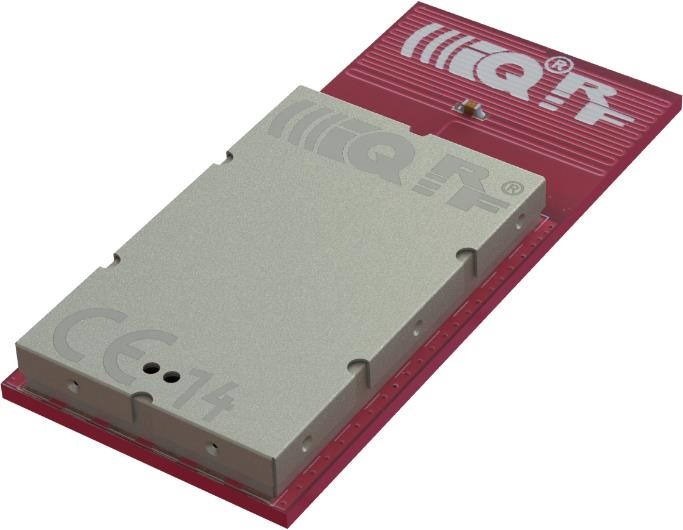
\includegraphics[width = 64mm]{img/iqrf/dctr-72dat.png}
\caption{Fotografie bezdrátového modulu}
\end{figure}

Modul může vysílat na bezlicenčních pásmech 916~MHz, která je určené pro Ameriku, a 868~MHz, určené pro zbytek světa. Vysílací výkon modulu je 12,5~mW, používá GFSK\index[zkr]{GFSK!Gaussian frequency-shift keying|textit} modulaci. Modul má integrovanou anténu na svém plošném spoji. \\

Pro komunikaci používá tzv. mesh neboli smíšenou topologii. Ta má výhody v~robustnosti a v~absenci centrálního prvku. Její nevýhodou je naopak potřebná ochrana proti zacyklení a nutnost směrování provozu. \\

Modul lze napájet napětím 3,1~V až 5,5~V, protože obsahuje LDO\index[zkr]{LDO!Low-dropout|textit} napěťový stabilizátor Microchip MCP1700T-3002E/TT. Dále modul obsahuje mikrokontrolér Microchip PIC16LF1938. Ten užívá operační systém IQRF OS, který za uživatele zajišťuje komunikaci s~integrovaným obvodem STMicroelectronics Spirit1. Tento obvod řídí bezdrátový datový přenos a má hardwarovou podporu blokové šifry AES-128\index[zkr]{AES!Advanced Encryption Standard|textit}. Operační systém dále ovládá integrované periferie (například digitální teploměr). IQRF DPA\index[zkr]{DPA!Direct Peripheral Access|textit} a uživatelská aplikace. Dále modul obsahuje digitální teploměr Microchip MCP9808E/MC. \\

Microchip PIC16LF1938 je 8-bitový mikrokontrolér s~architekturou PIC, která používá architekturu RISC\index[zkr]{RISC!Reduced instruction set computing|textit}, jenž má omezenou instruktážní sadu a rychlé vykonávání instrukcí. Flash paměť pro program má velikost 28~kB, paměť EEPROM má velikost 256~B a paměť SRAM má velikost 1~kB.

\begin{figure}[H]
\centering
\label{fig:iqrf/zjednodusene-schema}
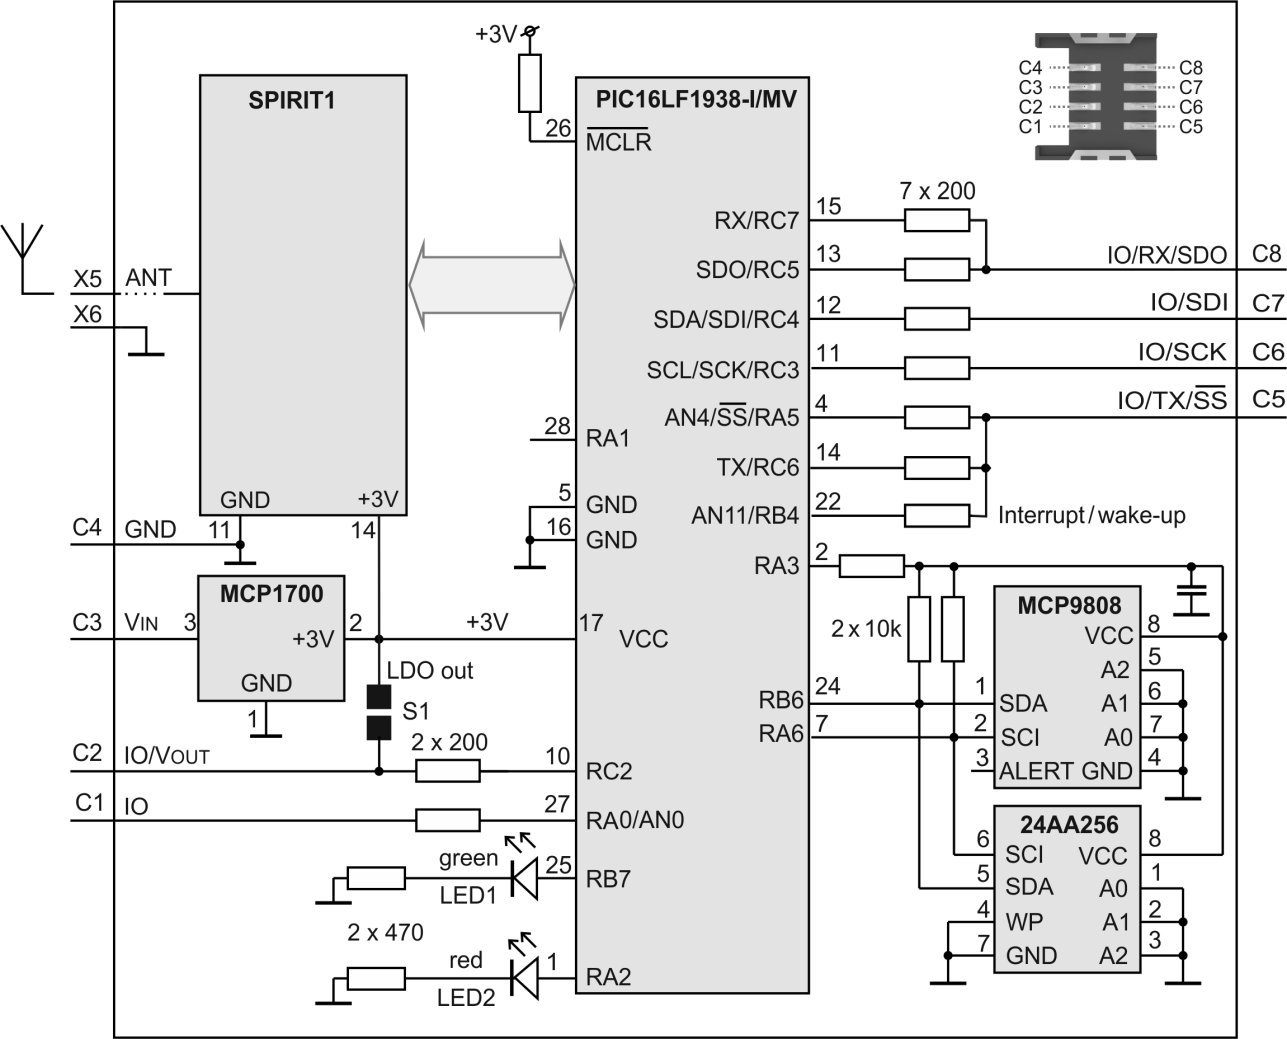
\includegraphics[width = 128mm]{img/iqrf/dctr-72dat-zjednodusene-schema.png}
\caption{Zjednodušené schéma bezdrátového modulu}
\end{figure}

\newpage

\subsection{Senzor teploty a vlhkosti}

\subsection{Regulátor PWM ventilátorů}

\subsection{Brána}

Jako bránu jsem použil jednodeskový počítač Raspberry Pi 3 model B. Bezdrátový modul IQRF DCTR-72DAT je k~bráně připojen přes sběrnici SPI\index[zkr]{SPI!Serial Peripheral Interface|textit} pomocí adaptéru IQRF KON-RASP-01. Brána se napájí pomocí externího spínaného zdroje s~microUSB konektorem, který má výstupní napětí 5~V a maximální výstupní proud 2~A.

\subsubsection{Raspberry Pi 3 model B}

Raspberry Pi 2 model B je jednodeskový počítač, který má rozměry podobné kreditní kartě. Tento počítač obsahuje:

\begin{itemize}
  \item čtyřjádrový ARM\index[zkr]{ARM!Acorn RISC Machine|textit}\index[zkr]{ARM!Advanced RISC Machine|textit} Cortex-A7 Broadcom BCM2837,
  \item 1~GB operační paměti RAM\index[zkr]{RAM!Random-access memory|textit},
  \item čtyři USB 2.0 porty
  \item port RJ45 pro 100~Mb síťovou kartu,
  \item slot pro microSD\index[zkr]{SD!Secure Digital|textit} kartu,
  \item HDMI\index[zkr]{HDMI!High-Definition Multimedia Interface|textit} výstup,
  \item 40 GPIO\index[zkr]{GPIO!General-purpose input/output|textit} pinů, na kterých jsou vyvedeny sběrnice SPI\index[zkr]{SPI!Serial Peripheral Interface|textit}, I2C\index[zkr]{I2C!Inter-Integrated Circuit|textit}, USART\index[zkr]{USART!Universal Synchronous / Asynchronous Receiver and Transmitter|textit}.
\end{itemize}

\begin{figure}[H]
\centering
\label{fig:foto/rpi2}
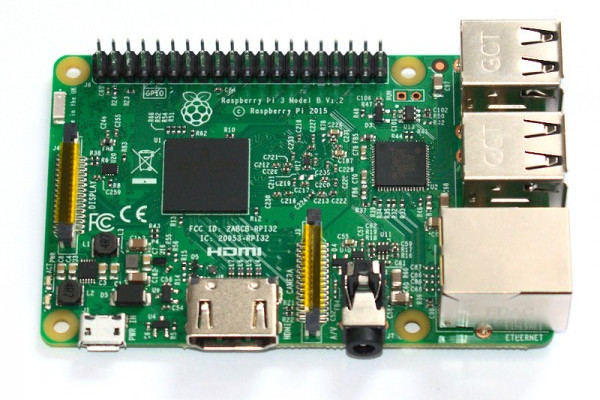
\includegraphics[width = 128mm]{img/foto/rpi3.jpg}
\caption{Fotografie jednodeskového počítače Raspberry Pi 3 model B}
\end{figure}

\newpage

\section{Návrh software}

\subsection{Komunikace}

\subsection{Senzor teploty a vlhkosti}

Software senzoru je psán v~programovacím jazyce C. Software byl napsán ve vývojovém prostředím IQRF IDE\cite{iqrf/ide}\index[zkr]{IDE!Integrated Development Environment|textit}.

\subsubsection{Vývojové prostředí IQRF IDE}

IQRF IDE\cite{iqrf/ide} je zdarma stažitelné vývojové prostředí, které je určené pro vývoj aplikací pro bezdrátové moduly IQRF. Toto vývojové prostředí je pouze pro operační systém Microsoft Windows. Uživatelé operačního systému Apple OS X nebo libovolné linuxové distribuce nemohou vyvíjet software pro tyto bezdrátové moduly. IQRF IDE používá kompilátor CC5X C Compiler\cite{cc5x-compiler}.

\begin{figure}[H]
\centering
\label{fig:iqrf/ide}
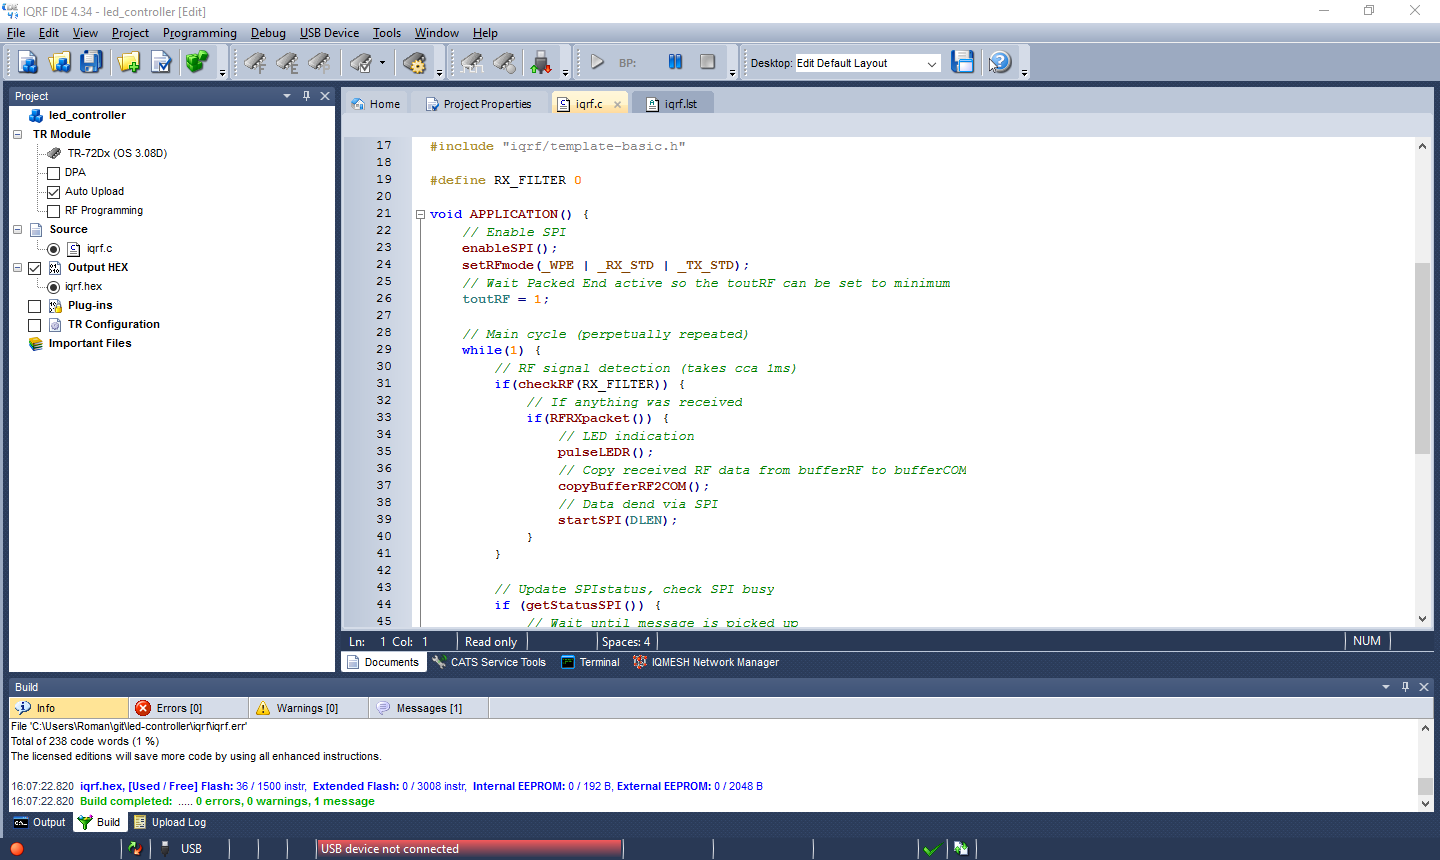
\includegraphics[width = 150mm]{img/iqrf/ide.png}
\caption{Vývojové prostředí IQRF IDE}
\end{figure}

\newpage

\subsubsection{Operační systém IQRF OS}

IQRF OS\cite{iqrf/os} je operační systém určený pro bezdrátové moduly IQRF, pomocí kterého může uživatel jednoduše:

\begin{itemize}
  \item ovládat rádiovou komunikaci,
  \item ovládat komunikaci v~mesh síti,
  \item komunikovat s~periferiemi přes sběrnice SPI, USART, I2C,
  \item pracovat s~pamětmi RAM\index[zkr]{RAM!Random-access memory|textit}, EEPROM\index[zkr]{EEPROM!Electrically Erasable Programmable Read-Only Memory|textit},
  \item inicializovat GPIO,
  \item spínat GPIO,
  \item číst logické hodnoty z~GPIO,
  \item spínat integrované LED\index[zkr]{LED!Light-Emitting Diode|textit} diody,
  \item generovat PWM\index[zkr]{PWM!Pulse Width Modulation|textit} na výstupním pinu,
  \item číst hodnoty z~analogově digitálního převodníku,
  \item číst teplotu z~integrovaného teplotního senzoru.
\end{itemize}

\begin{figure}[H]
\centering
\label{fig:foto/iqrf-os}
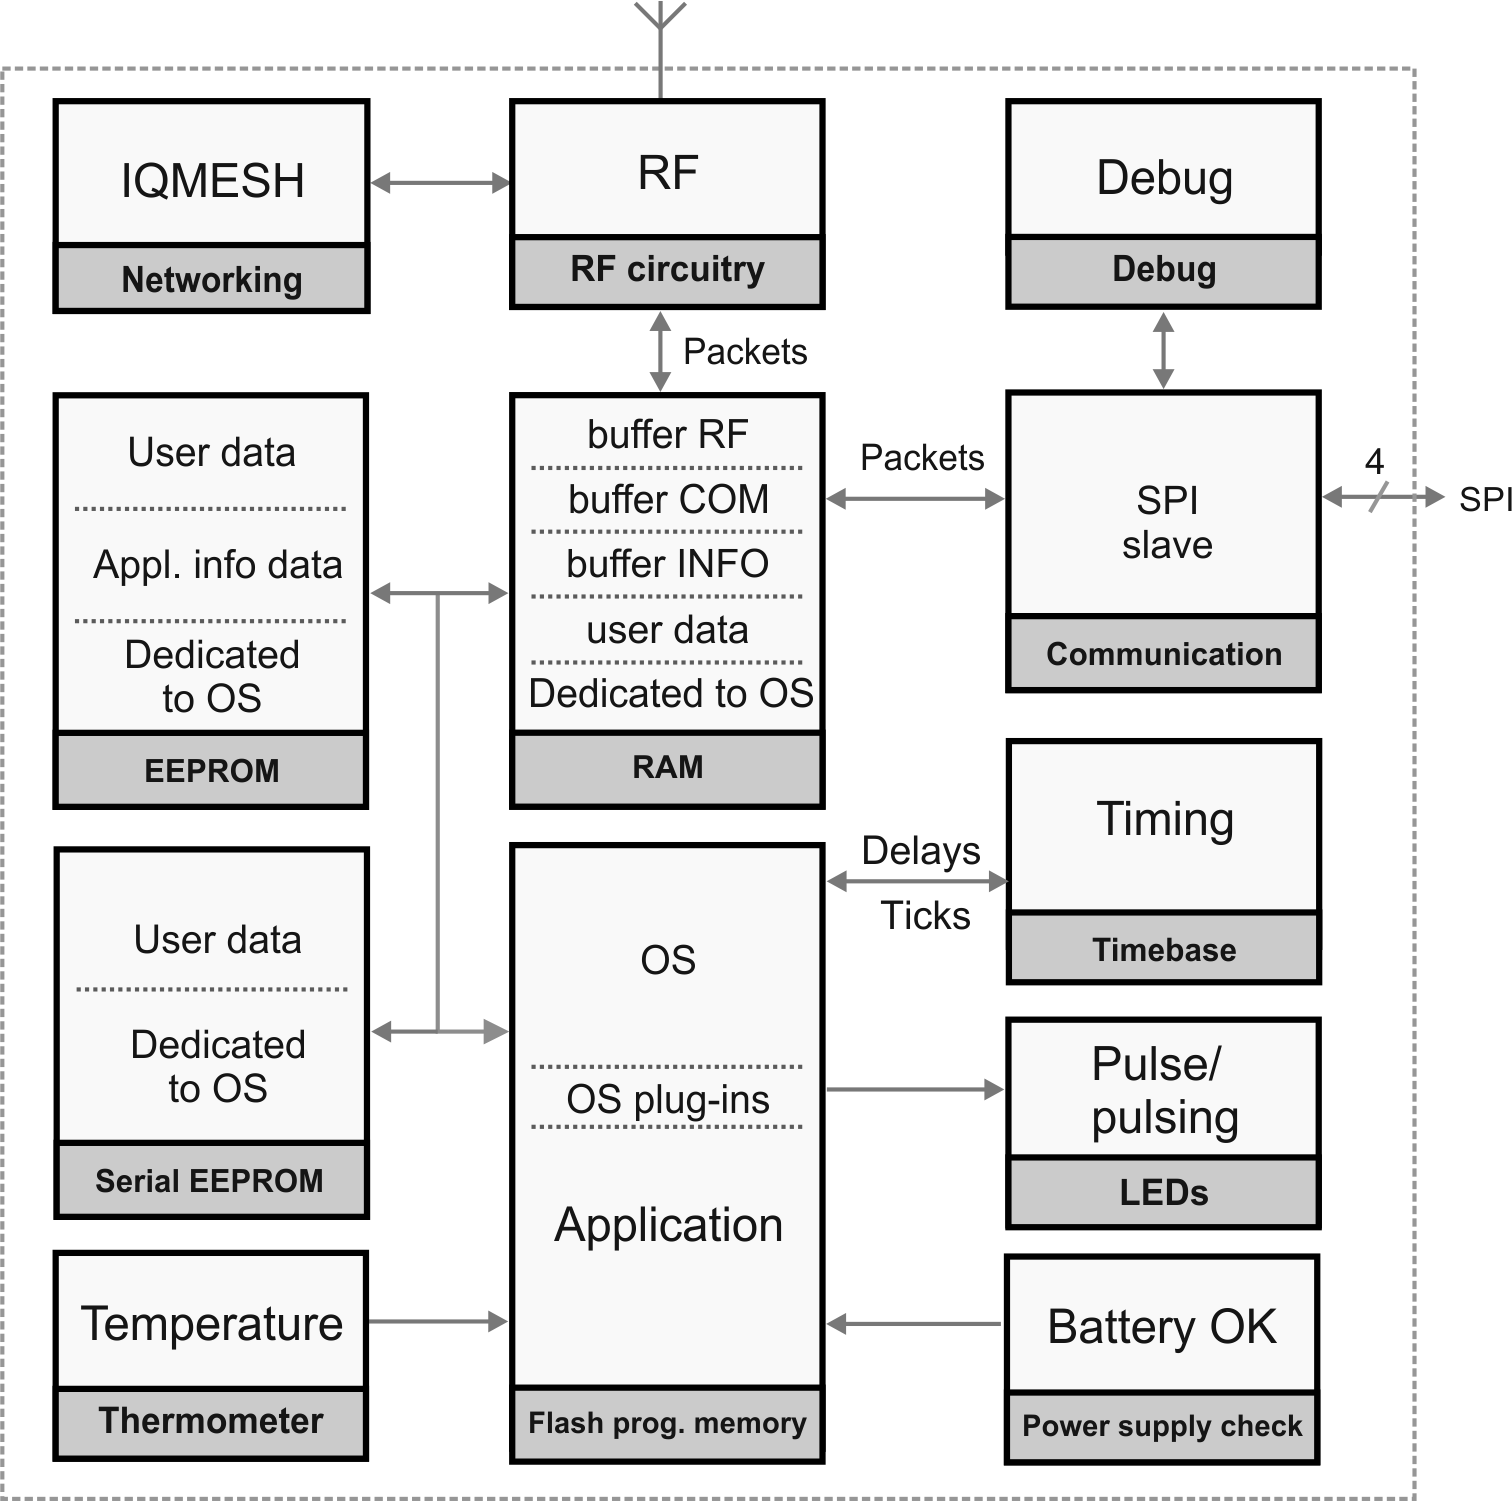
\includegraphics[width = 100mm]{img/iqrf/os-blokove-schema.png}
\caption{Blokové schéma operačního systému IQRF OS}
\end{figure}

\newpage

\subsubsection{Protokol IQRF DPA}

IQRF DPA\cite{iqrf/dpa} je vrstva nad IQRF OS, která se stará o~protokol komunikace IQRF bezdrátových modulů. IQRF DPA má pevně danou strukturu paketů, která je uvedena v~tabulce č.~3. Centrální prvek v~IQRF mesh síti se jmenuje koordinátor, který je umístěn v~bráně. Koordinátor má se své paměti EEPROM uložené informace o~dalších bezdrátových modulech, se kterými má komunikovat. Pokud koordinátor přijme data od bezdrátového modulu, jehož informace nemá uložené v~EEPROM paměti, pak data ignoruje.

\begin{table}[H]
\centering
\begin{tabular}{|c|c|c|c|c|}
\hline
NADR & PNUM & PCMD & HWPID & DATA \\
\hline
siťová adresa & číslo periferie & příkaz & HWP\index[zkr]{HWP!Hardware profile|textit} identifikátor & data \\
\hline
\end{tabular}
\caption{Schéma paketu IQRF DPA}\label{table:iqrf/dpa}
\end{table}

\newpage

\subsection{Brána}

V~bráně běží linuxová distribuce Raspbian, což je speciálně upravená linuxová distribuce pro jednodeskový počítač Raspberry Pi. Tato linuxová distribuce je odvozená od linuxové distribuce Debian, která je jedna z~nejpoužívanějších linuxových distribucích. \\
Pro komunikaci s IQRF sítí je použit IQRF Gateway Daemon\cite{iqrfsdk/iqrf-daemon}, což je open source software pod licencí Apache License 2.0 vyvíjený firmou IQRF Tech s.r.o., který obstarává komunikaci mezi IQRF sítí a MQTT brokerem. \\
Pro uživatelsky přívětivou konfiguraci IQRF Gateway Daemonu jsem vytvořil webovou aplikaci\cite{iqrfsdk/iqrf-daemon-webapp}, která je napsaná ve skriptovacím jazyce PHP s použitím českého frameworku Nette\cite{nette}.

\begin{figure}[H]
\centering
\label{fig:foto/iqrf-os}
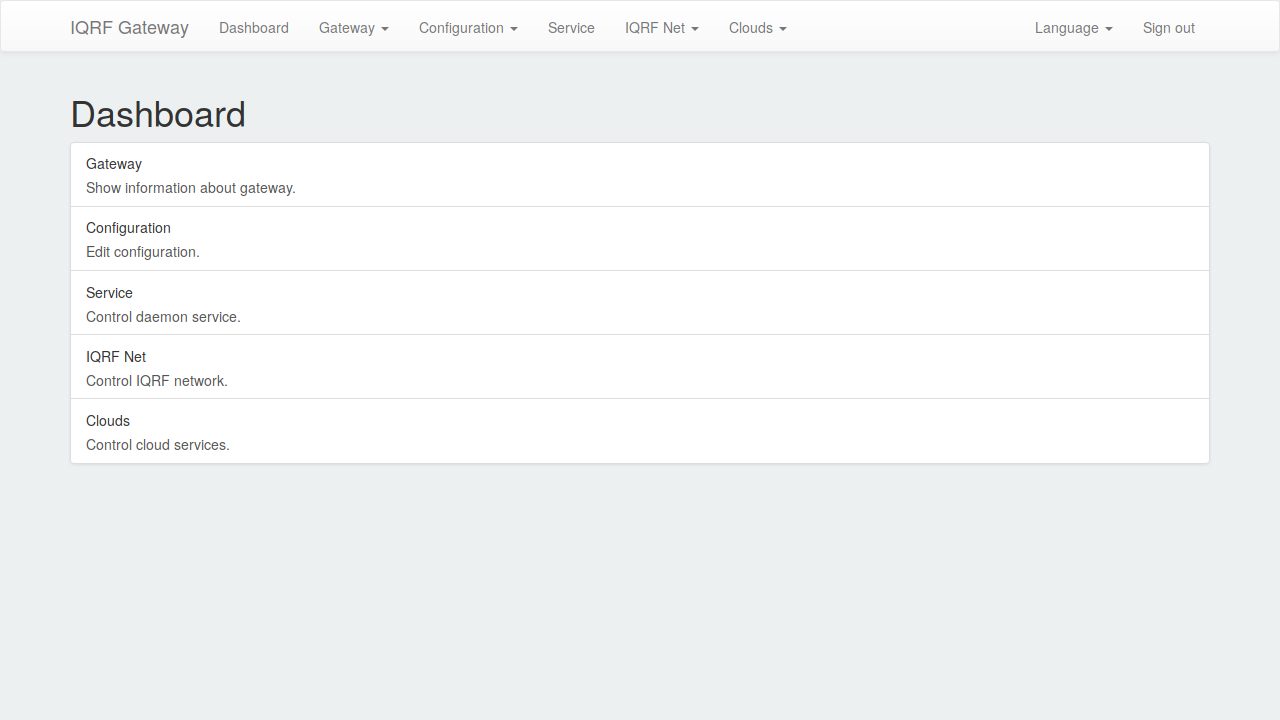
\includegraphics[width = 150mm]{img/iqrf/iqrf-daemon-webapp.png}
\caption{Výchozí stránka IQRF Gateway Daemon webapp}
\end{figure}

\newpage

\section{Technické parametry}

\newpage

\section*{Závěr}

\addcontentsline{toc}{section}{Závěr}

\newpage

\printindex[zkr]

\addcontentsline{toc}{section}{Seznam použitých zkratek}

\newpage

\begin{thebibliography}{99}

\addcontentsline{toc}{section}{Seznam použité literatury}

\bibitem{iqrf/ide}
IQRF Tech s.r.o.. IQRF IDE \emph{IQRF} [online]. Jičín, 2018 [cit. 2018-02-19]. \\ Dostupné z: \url{https://www.iqrf.org/technology/iqrf-ide}

\bibitem{iqrf/os}
IQRF Tech s.r.o.. Operating system \emph{IQRF} [online]. Jičín, 2018 [cit. 2018-02-19]. \\ Dostupné z: \url{https://www.iqrf.org/technology/operating-system}

\bibitem{iqrf/os/guide}
IQRF Tech s.r.o.. IQRF OS v4.02D User's guide for TR-7xD \emph{IQRF} [online]. Jičín, 2017 [cit. 2018-02-19]. \\ Dostupné z: \url{http://www.iqrf.org/support/download&kat=35&ids=155}

\bibitem{iqrf/dpa}
IQRF Tech s.r.o.. DPA \emph{IQRF} [online]. Jičín, 2018 [cit. 2018-02-19]. \\ Dostupné z: \url{https://www.iqrf.org/technology/dpa}

\bibitem{iqrf/dpa/guide}
IQRF Tech s.r.o.. DPA Framework Technical guide v3.02 \emph{IQRF} [online]. Jičín, 2017 [cit. 2018-02-19]. \\ Dostupné z: \url{http://www.iqrf.org/support/download&kat=35&ids=155}

\bibitem{iqrf/dctr-72d-datasheet}
IQRF Tech s.r.o.. Datasheet (DC)TR-72D \emph{IQRF} [online]. Jičín, 2017 [cit. 2018-02-19]. \\ Dostupné z: \url{http://iqrf.org/weben/downloads.php?id=337}

\bibitem{iqrf/kon-rasp-01-datasheet}
IQRF Tech s.r.o.. User's guide KON-RASP-01 \emph{IQRF} [online]. Jičín, 2015 [cit. 2018-02-19]. \\ Dostupné z: \url{http://www.iqrf.org/weben/downloads.php?id=412}

\bibitem{iqrfsdk/iqrf-daemon}
IQRF Tech s.r.o.. IQRF Gateway Daemon \emph{IQRF} [online]. Jičín, 2018 [cit. 2018-02-19]. \\ Dostupné z: \url{https://github.com/iqrfsdk/iqrf-daemon}

\bibitem{iqrfsdk/iqrf-daemon-webapp}
IQRF Tech s.r.o.. IQRF Gateway Daemon webapp \emph{IQRF} [online]. Jičín, 2018 [cit. 2018-02-19]. \\ Dostupné z: \url{https://github.com/iqrfsdk/iqrf-daemon-webapp}

\bibitem{nette}
Nette Foundation. Nette Framework \emph{Nette} [online]. Praha, 2018 [cit. 2018-02-19]. \\ Dostupné z: \url{https://nette.org/}

\bibitem{rpi3-spec}
Raspberry Pi Foundation. Raspberry Pi 3 Model B Specifications \emph{Raspberry Pi} [online]. UK, 2018 [cit. 2018-02-19]. \\ Dostupné z: \url{https://www.raspberrypi.org/products/raspberry-pi-3-model-b/}

\end{thebibliography}

\newpage

\listoffigures

\addcontentsline{toc}{section}{Seznam obrázků}

\listoftables

\addcontentsline{toc}{section}{Seznam tabulek}

\end{document}